\documentclass[11pt]{beamer}
\usetheme{Madrid}
\usepackage[utf8]{inputenc}
\usepackage[francais]{babel}
\usepackage[T1]{fontenc}
\usepackage{amsmath}
\usepackage{amsfonts}
\usepackage{amssymb}
\usepackage{graphicx}
\usepackage{tikz}
\title[\'Equation d'advection sur la sphère]{Schémas au différences compacts pour la résolution de l'équation d'advection sphérique\\
\small{Séminaire Doctorants de Strasbourg}}
\setbeamercovered{transparent} 
\setbeamertemplate{navigation symbols}{} 
\author{Brachet Matthieu}
\logo{IECL.jpg} 
\date[17.03.2017]{Jeudi 17 Mars 2016}
\institute[IECL]{Institut Elie Cartan de Lorraine}
%\subject{} 
\begin{document}

\begin{frame}
\titlepage
\begin{center}

\includegraphics[width=2.5cm]{IECL.jpg}
\end{center}
\end{frame}


\section{Introduction}
\begin{frame}{Introduction}
  \begin{block}{Objectif :}
    Résolution numérique d'EDP sur la sphère.
  \end{block}
\begin{figure}
\begin{center}
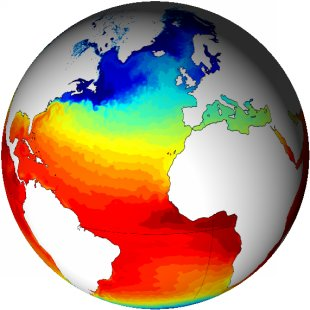
\includegraphics[scale=0.22]{oceanographie.jpg}
\hspace{2cm}
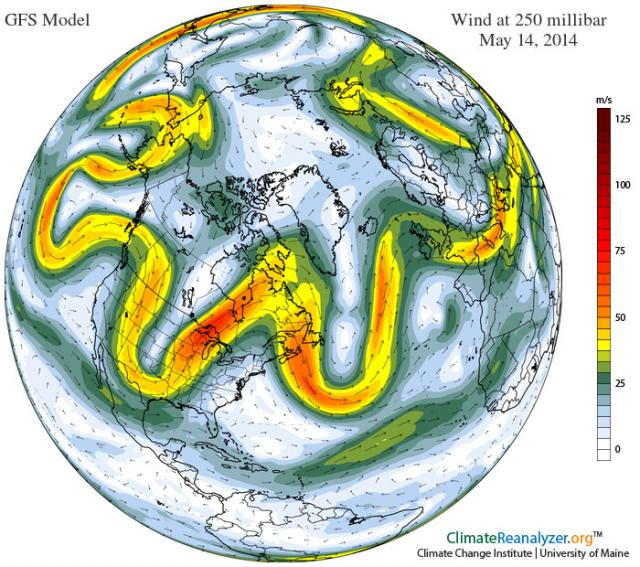
\includegraphics[scale=0.12]{climato.jpg}
\caption{(gauche) Océanographie(Image Mercator océan) - (droite)
  Jet-Stream(ClimateReanalyzer.org$^{TM}$)}
\end{center}
\end{figure}
\end{frame}

\begin{frame}
\begin{columns}
% ***
\column{0.45\textwidth}
  Méthodes déjà existantes :
  \begin{itemize}
    \item Problème des pôles
    \item Rapidité du calcul
    \item Précision
  \end{itemize}
% ***
\column{0.45\textwidth}
\begin{figure}
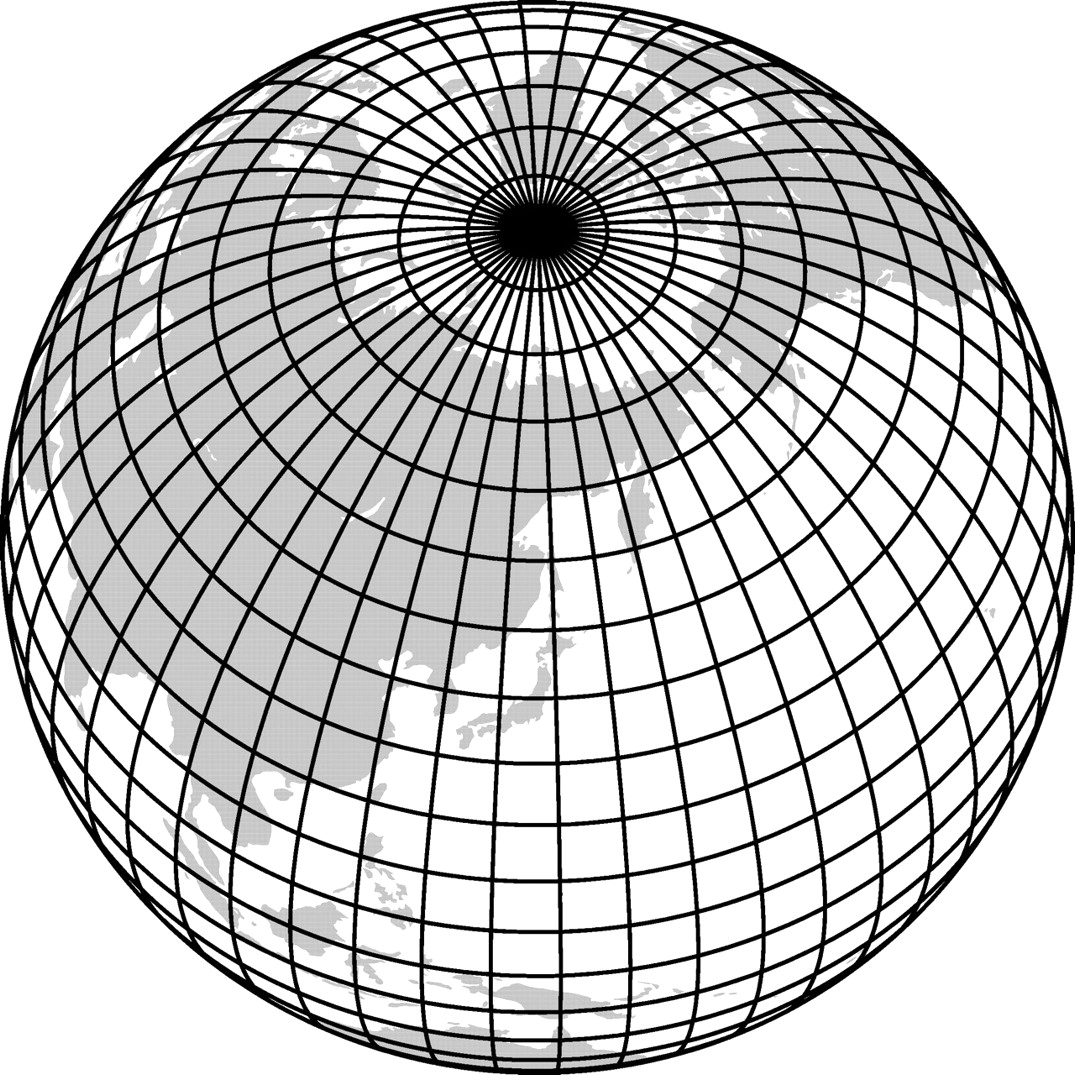
\includegraphics[height=3cm]{lonlat_grid.jpg}
\caption{Maillage Longitude/Latitude}
\end{figure}
\end{columns}
\pause

  \begin{exampleblock}{Dans cet exposé :}
    \begin{itemize}
    \item Présentation de la méthode de discrétisation spaciale : rapide et précis en différences finies;
    \item Discrétisation temporelle : Runge Kutta avec filtrage des hautes fréquences.  
    \end{itemize}
  \end{exampleblock}
\end{frame}




% ********************************************************************************

\begin{frame}
\tableofcontents
\end{frame}

% ********************************************************************************

\section{Calcul du gradient sphérique}
\subsection{Maillage Cube-Sphère}
\begin{frame}{Maillage "Cube-Sphere"}

\begin{exampleblock}{Idée (Croisille (2014)):}
Construire une méthode rapide, précise et efficace pour calculer des opérateurs différentiels sur la sphère.
\end{exampleblock}

\pause

\begin{columns}

\column{0.45\textwidth}
Poles :
\begin{itemize}
\item Nord : $N (0,0,R)$,
\item Sud : $S (0,0,-R)$.
\end{itemize}

\begin{center}
\begin{tikzpicture}[scale=1.2]
    \draw (0,1) node {$\bullet$} ;
	\draw (0,1) node[above]{$N$} ;
	\draw (0,-1) node {$\bullet$} ;
	\draw (0,-1) node[below]{$S$} ;
    \draw (0,1) arc (90:270:0.75cm and 1cm);
    \draw (0,1) arc (90:270:0.50cm and 1cm);
    \draw (0,1) arc (90:270:0.25cm and 1cm);
    \draw (0,1) arc (90:270:0cm and 1cm);
    \draw (0,1) arc (90:-90:0.25cm and 1cm);
    \draw (0,1) arc (90:-90:0.50cm and 1cm);
    \draw (0,1) arc (90:-90:0.75cm and 1cm);    
    \draw (0,0) circle (1cm);
    \shade[ball color=blue!10!white,opacity=0.20] (0,0) circle (1cm);
\end{tikzpicture}
\end{center}

\pause

\column{0.45\textwidth}
Poles :
\begin{itemize}
\item East : $E (0,R,0)$,
\item West : $W (0,-R,0)$.
\end{itemize}
\begin{center}
\begin{tikzpicture}[scale=1.2]
	\draw (1,0) node {$\bullet$} ;
	\draw (1,0) node[right]{$E$} ;
	\draw (-1,0) node {$\bullet$} ;
	\draw (-1,0) node[left]{$W$} ;   
    \draw (-1,0) arc (180:360:1cm and 0.75cm);
    \draw (-1,0) arc (180:360:1cm and 0.25cm);
    \draw (-1,0) arc (180:360:1cm and 0.5cm);
    \draw (-1,0) arc (180:360:1cm and 0cm);
    \draw (-1,0) arc (180:360:1cm and -0.25cm);
    \draw (-1,0) arc (180:360:1cm and -0.5cm);
    \draw (-1,0) arc (180:360:1cm and -0.75cm);    
    \draw (0,0) circle (1cm);
    \shade[ball color=blue!10!white,opacity=0.20] (0,0) circle (1cm);
\end{tikzpicture}
\end{center}
\end{columns}
\end{frame}

\begin{frame}
\begin{exampleblock}{}
Création d'un maillage couvrant une partie de la sphère.
\end{exampleblock}
\begin{figure}
\begin{columns}
\column{0.45\textwidth}
\begin{center}
\begin{tikzpicture}[scale=1.2]
    \draw (-0.60,-0.60) arc (225:315:0.85cm and 0.50cm);
    \draw (-0.74,-0.17) arc (210:331:0.85cm and 0.16cm);
    \draw (-0.705,-0.35) arc (225:314:1cm and 0.5cm);
    \draw (-0.75,0) arc (180:360:0.75cm and 0cm);    
    \draw (0.74,0.17) arc (30:151:0.85cm and 0.16cm);
    \draw (0.705,0.35) arc (45:135:1cm and 0.5cm);
    \draw (0.60,0.60) arc (45:135:0.85cm and 0.50cm);
    \draw (0.60,-0.60) arc (-45:45:0.51cm and 0.85cm);
    \draw (0.17,-0.74) arc (-60:60:0.16cm and 0.85cm);
    \draw (0.35,-0.705) arc (-58:60:0.3cm and 0.82cm);
    \draw (0,0.75) arc (90:270:0cm and 0.75cm);
    \draw (-0.60,0.60) arc (135:225:0.51cm and 0.85cm);
    \draw (-0.17,0.74) arc (120:240:0.16cm and 0.85cm);
    \draw (-0.35,0.705) arc (122:240:0.3cm and 0.82cm);    
    \draw (0,0) circle (1cm);
    \draw (0.60,0.60) -- (0.707,0.707) ;
    \draw (-0.60,0.60) -- (-0.707,0.707) ;
    \draw (0.60,-0.60) -- (0.707,-0.707) ;
    \draw (-0.60,-0.60) -- (-0.707,-0.707) ;
    \shade[ball color=blue!10!white,opacity=0.20] (0,0) circle (1cm);
\end{tikzpicture}
\end{center}
\column{0.45\textwidth}
\begin{center}
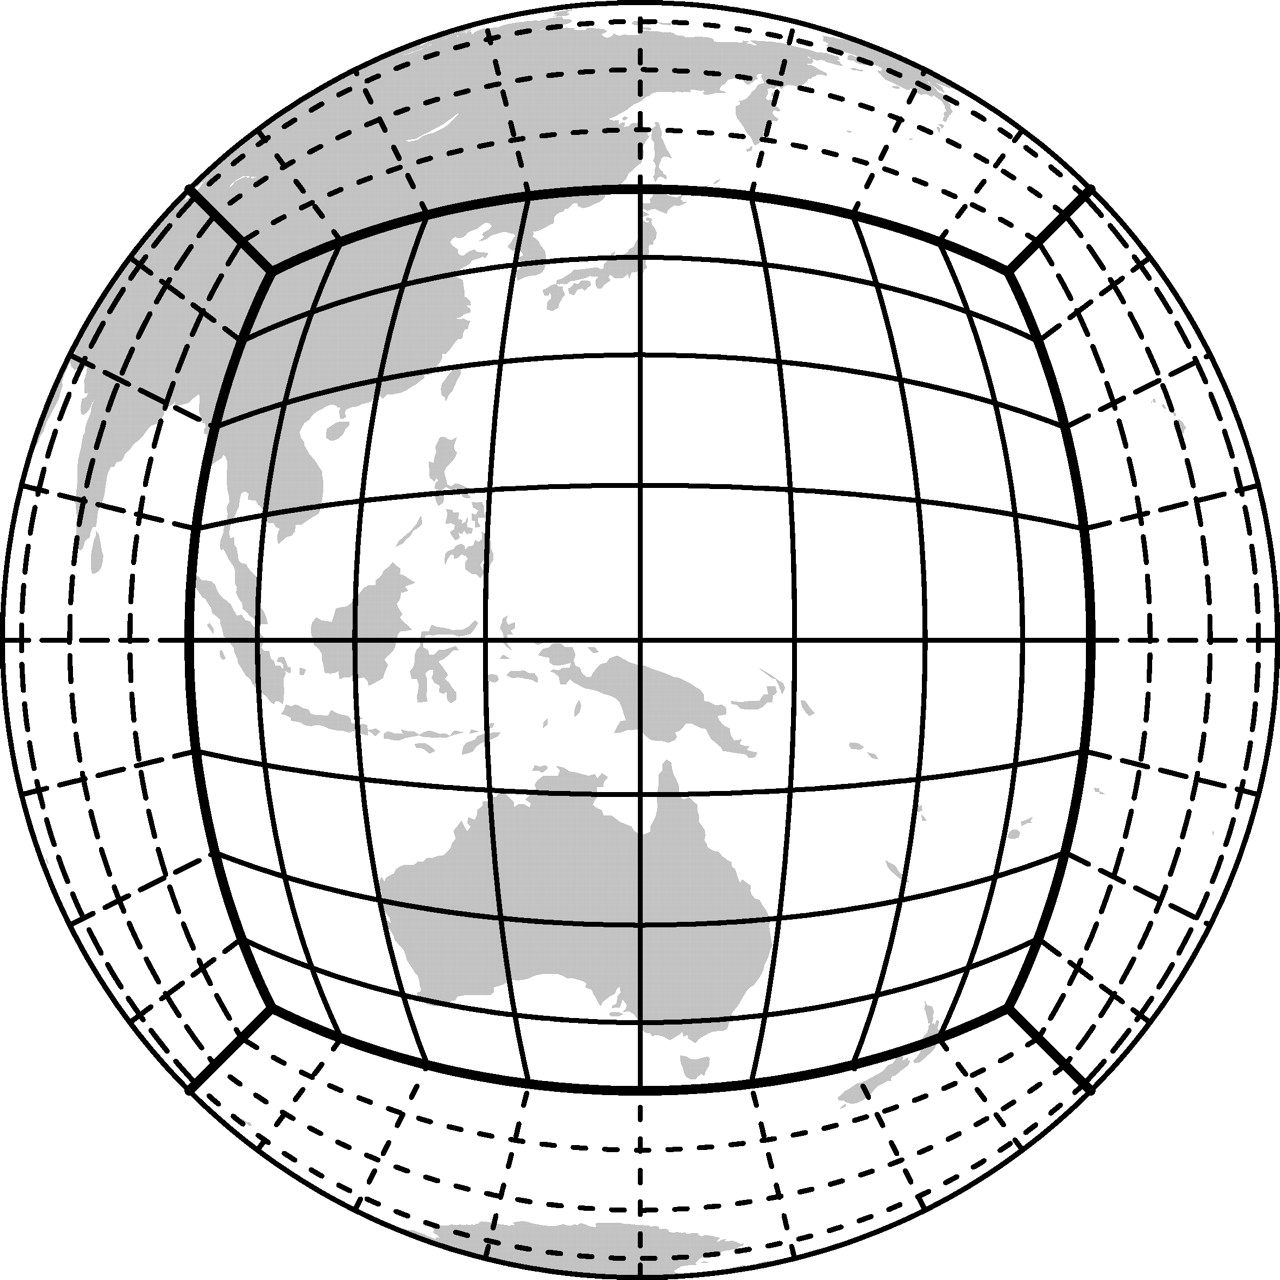
\includegraphics[scale=0.055]{CS_grid.jpg}
\end{center}
\end{columns}
\caption{Cube-Sphere - Front (gauche) et Complet (droite)}
\end{figure}
\end{frame}

% ********************************************************************************
\begin{frame}{Coordonnées}
\begin{columns}
\begin{column}{5cm}
\begin{figure}
\begin{tikzpicture}[scale=1.8]
	\draw (0,0) node {$\bullet$} ;
	\draw [>=stealth, ->] (0,0) -- (1.5,0) ; 
	\draw (1.5,0) node[above right]{$y$} ;   
	\draw [>=stealth, ->] (0,0) -- (1.1,-0.8) ; 
	\draw (1.1,-0.8) node[above right]{$x$} ; 
	\draw [>=stealth, ->] (0,0) -- (0,1.5) ; 
        \draw (0,1.5) node[above right]{$z$} ; 

        \draw[color=green] (0.065,0.5) arc (85:68:1cm and 0.5cm);
        \draw[color=green] (0.2,0.55) node{$\alpha$} ;
        \draw[color=red] (0.4,-0.05) arc (-5:25:0.41cm and 1cm);
        \draw[color=red] (0.48,0.2) node{$\beta$} ;
        \draw (-1,0)[dotted, color=black!40] arc (180:360:1cm and -0.5cm);
        \draw (0,1)[dotted, color=black!40] arc (90:270:-0.4cm and 1cm);
        \draw (-1,0)[dotted, color=black!20] arc (180:360:1cm and 0.5cm);
        \draw (0,1)[dotted, color=black!20] arc (90:270:0.4cm and 1cm);
    
        \draw (-1,0) arc (180:360:1cm and 0.06cm);
        \draw (0,1) arc (90:270:-0.08cm and 1cm);
        \draw[dashed] (-1,0) arc (180:360:1cm and -0.06cm);
        \draw[dashed] (0,1) arc (90:270:0.08cm and 1cm);
    
        \draw (0.36,0.46) node {$\bullet$} ;
	\draw (0.36,0.46) node[above right]{$M$} ;
        \draw (0,0) circle (1cm);
    \shade[ball color=blue!10!white,opacity=0.20] (0,0) circle (1cm);
\end{tikzpicture}
\caption{Coordonnées sur la CS}
\end{figure}
\end{column}
\pause
\begin{column}{5cm}
Dans ce système de coordonnées $M$ est donné par :

\begin{itemize}
\item $\alpha$ abscisse curviligne le long du grand cercle "horizontal".

\item $\beta$ abscisse curviligne le long du grand cercle "vertical".

\item $\xi$ angle equatiorial partant du centre du patch.

\item $\eta$ angle latitudinal partant du centre du patch.
\end{itemize}
\end{column}
\end{columns}


\end{frame}


\begin{frame}{Calcul du gradient sphèrique}
Gradient :
$$\nabla_T u = \dfrac{\partial u}{\partial \xi}_{|\eta} g^\xi + \dfrac{\partial u}{\partial \eta}_{|\xi} g^\eta $$

$\rightarrow$ $\dfrac{\partial u}{\partial \xi}_{|\eta}$ et $\dfrac{\partial u}{\partial \eta}_{|\xi}$ : pas le long des grands cercles. Exprimer dans $(\alpha, \beta)$.
\pause
\begin{block}{Gradient sur la CS}
$$\nabla_T u = \frac{\partial u}{\partial \alpha}_{|\eta} \left( \cos \eta \dfrac{1+ \tan^2 \xi}{1 + \cos^2 \eta \tan^2 \xi} \right) g^\xi + \frac{\partial u}{\partial \beta}_{|\xi} \left( \cos \xi \dfrac{1+ \tan^2 \eta}{1 + \cos^2 \xi \tan^2 \eta} \right) g^\eta $$
\end{block}
\pause
$\rightarrow$ Évaluer $\dfrac{\partial u}{\partial \alpha}_{|\eta}$ et $\dfrac{\partial u}{\partial \beta}_{|\xi}$ en chaque point du maillage.
\end{frame}



\subsection{Schémas compacts hermitiens}

\begin{frame}{Schémas compacts hermitiens}
\begin{exampleblock}{Problèmatique :}
Evaluer la dérivée première par différence finies.
\end{exampleblock}

\pause

\textbf{Schémas classiques :}

$$\partial_x u(x) = \sum_{p=1}^N a_p \dfrac{ u(x+ph) - u(x_ph)}{2ph} +
\mathcal{O}\left( h^{\alpha} \right)$$

Exemples :
\begin{itemize}
\item $\partial_x u(x) = \dfrac{u(x+h) - u(x-h)}{2h} +
  \mathcal{O}(h^2)$
\item  $\partial_x u(x) = \dfrac{4}{3}\dfrac{u(x+h) - u(x-h)}{2h} - \dfrac{1}{3}\dfrac{u(x+2h) - u(x-2h)}{4h} + \mathcal{O}(h^4)$
\end{itemize}

\end{frame}


\begin{frame}{Schémas compacts hermitiens}
\begin{exampleblock}{Problèmatique :}
Evaluer la dérivée première par différence finies.
\end{exampleblock}

\pause

\textbf{Schémas compacts (Lele (1992)):}

<<<<<<< HEAD
\small{$$\partial_x u(x) + \sum_{j=1}^M \alpha_j \left( \partial_x u(x+jh)+\partial_x u(x-jh)\right) = \sum_{p=1}^N a_p \dfrac{ u(x+ph) - u(x_ph)}{2ph} +
=======
\small{$$\alpha_0 \partial_x u(x) + \sum_{j=1}^M \alpha_j \left( \partial_x u(x+jh)+\partial_x u(x-jh)\right) = \sum_{p=1}^N a_p \dfrac{ u(x+ph) - u(x_ph)}{2ph} +
>>>>>>> ca5c7bdbcc04225aecffb2770e2b9cef792c57cd
\mathcal{O}\left( h^{\alpha} \right)$$}

Exemple :
\begin{itemize}
\item $\dfrac{2}{3} \partial_x u(x) + \dfrac{1}{6} \left( \partial_x
  u(x+h) + \partial_x u(x-h) \right) = \dfrac{u(x+h) - u(x-h)}{2h} + \mathcal{O} \left( h^4 \right) $
\end{itemize}

\end{frame}






\begin{frame}
\begin{alertblock}{}
Quel intér\^et?
\end{alertblock}
\pause
\begin{block}{}
Meilleur représentation des hautes fréquences
\end{block}

\begin{columns}
\column{0.45\textwidth}
\textbf{Nombre d'onde exacte :}

$$\mathcal{F}\left( \partial_x u \right) = i \dfrac{\theta}{h} \mathcal{F}\left( u \right)$$

avec $\theta = h \xi$.

\column{0.45\textwidth}
\textbf{Nombre d'onde approché :}
$$\mathcal{F}\left( \delta_x u \right) = i \dfrac{\theta_m}{h}
\mathcal{F}\left( u \right)$$

où $\theta_m$ est obtenu à partir du schéma en différences finies utilisé.
\end{columns}
\vspace{0.8cm}
\pause
$$\theta_m = \dfrac{\sum_{p=1}^N a_p sin( p \theta )}{\alpha_0 + 2
  \sum_{j=1}^M \alpha_j cos(j \theta)}$$


\end{frame}

\begin{frame}
\begin{figure}
\begin{center}
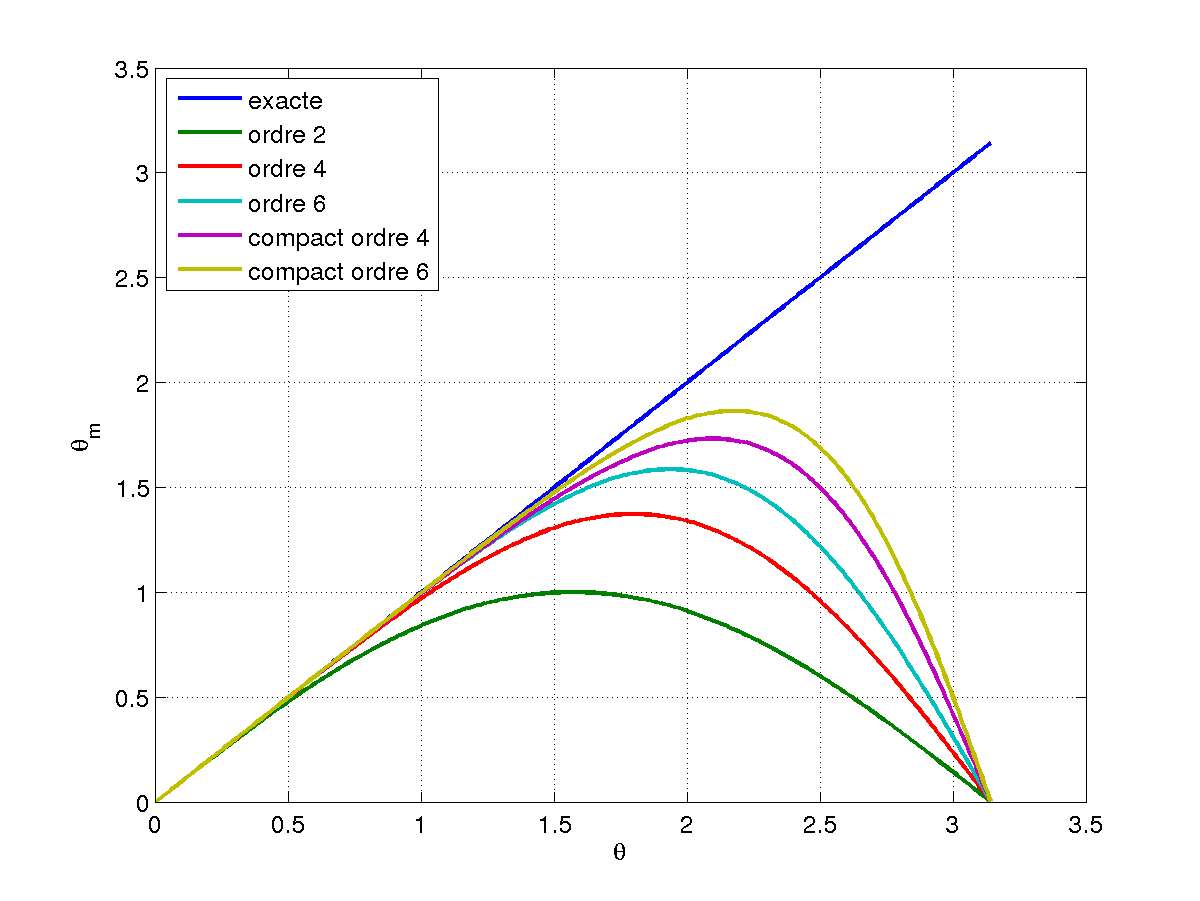
\includegraphics[scale=0.4]{onde_modifiee.png}
\caption{Nombre d'onde modifiée}
\end{center}
\end{figure}

\end{frame}

\subsection{Résultats numériques}
\begin{frame}{Résultats numériques}
Soit $u(x,y,z) = sin(10 \pi x)sin(2 \pi y) sin(6 \pi z)$, avec
$(x,y,z) \in \mathbb{S}^1$

erreur :

$$e_{\infty} = max | (\nabla_T u)_{app} - (\nabla_T u)_{ex} |$$

<<<<<<< HEAD
$N$ : nombre de points par face de la Cube-Sphere.
=======
$N$ : paramètre de discrétisation.
>>>>>>> ca5c7bdbcc04225aecffb2770e2b9cef792c57cd

\begin{center}
\tiny{\begin{tabular}{|c||c|c|c|c|c|c|c|c|c|}
\hline 
 & $N=8$ & taux & $N=16$ & taux & $N=32$ & taux & $N=64$ & taux & $N=128$ \\ 
\hline 
\hline
$e_{\infty}$ & $23.475$ & $2.99$ & $2.949$ & $4.61$ & $0.121$ & $4.07$ & $7.205(-3)$ & $3.91$ & $4.774(-4)$ \\ 
\hline 
Nb pts & $386$ &  & $1538$ &  & $6146$ &  & $24578$ &  &
$93306$\\
\hline
\end{tabular} }
\end{center}

\end{frame}


% ********************************************************************************
\section{Méthodes de Runge-Kutta}

\subsection{Notions générales}
\begin{frame}{Notions générales}
Résolution de $$\dfrac{du}{dt} = f(t,u)$$ (avec C.I.).

\begin{block}{}
Méthode de Runge-Kutta :
\begin{itemize}
\item basée sur :
$$u(t) = \int^t f(\tau,y(\tau))d\tau$$
\item Méthode à un pas,
\item Possibilité d'obtenir de l'ordre élevé.
\item Co\^ut en calcul des méthodes implicites potentiellement très important.
\end{itemize}
\end{block}

\end{frame}

\begin{frame}
\begin{columns}
\column{0.52\textwidth}
\begin{block}{\textbf{Algorithme :}}

Pour $i=1...p$
\[
\left \{
\begin{array}{r @{=} l}
    t_{n,i} & t_n + c_i h \\
    y_{n,i} & y_n + h \sum_{k=1}^q a_{i,k}f(t_{n,k} , y_{n,k}) \\
    p_{n,i} & f( t_{n,i} , y_{n,i} )
\end{array}
\right.
\]

$$y_{n+1} = y_n + h \sum_{k=1}^q b_k p_{n,k}$$
\end{block}

\pause
\column{0.38\textwidth}
\begin{block}{\textbf{Tableau de Butcher :}}

\begin{tabular}{c|c}
$c$ & $A$\\
\hline
    & $b^T$
\end{tabular}

avec $A=(a_{i,k})_{i,k}$,

$b=(b_k)_k$,

et $c=(c_i)_i$.
\end{block}
\end{columns}

\end{frame}

\begin{frame}
\begin{block}{Méthode explicite (RK)}
\begin{itemize}
\item $a_{i,k} = 0$ si $i > k$;
\item Calcul direct à chaque étape.
\end{itemize}
\end{block}

\begin{block}{Méthode semi-implicites (DIRK)}
\begin{itemize}
\item $a_{i,k} = 0$ si $i \geq k$;
\item Une équation à une inconnue à résoudre à chaque étape,
\item Stabilité supérieure et plus grandes possibilités d'ordre.
\end{itemize}
\end{block}

\end{frame}

\subsection{Stabilité}
\begin{frame}{Stabilité}
Soit :
$$u' = \lambda u$$
Zone de stabilité d'une méthode de Runge Kutta :
$$Stab_{RK} = \lbrace z = h \lambda \in \mathbb{C} \text{ s. t. }
| u_{n+1} | \leq | u_n | \rbrace $$

\begin{figure}
\begin{center}
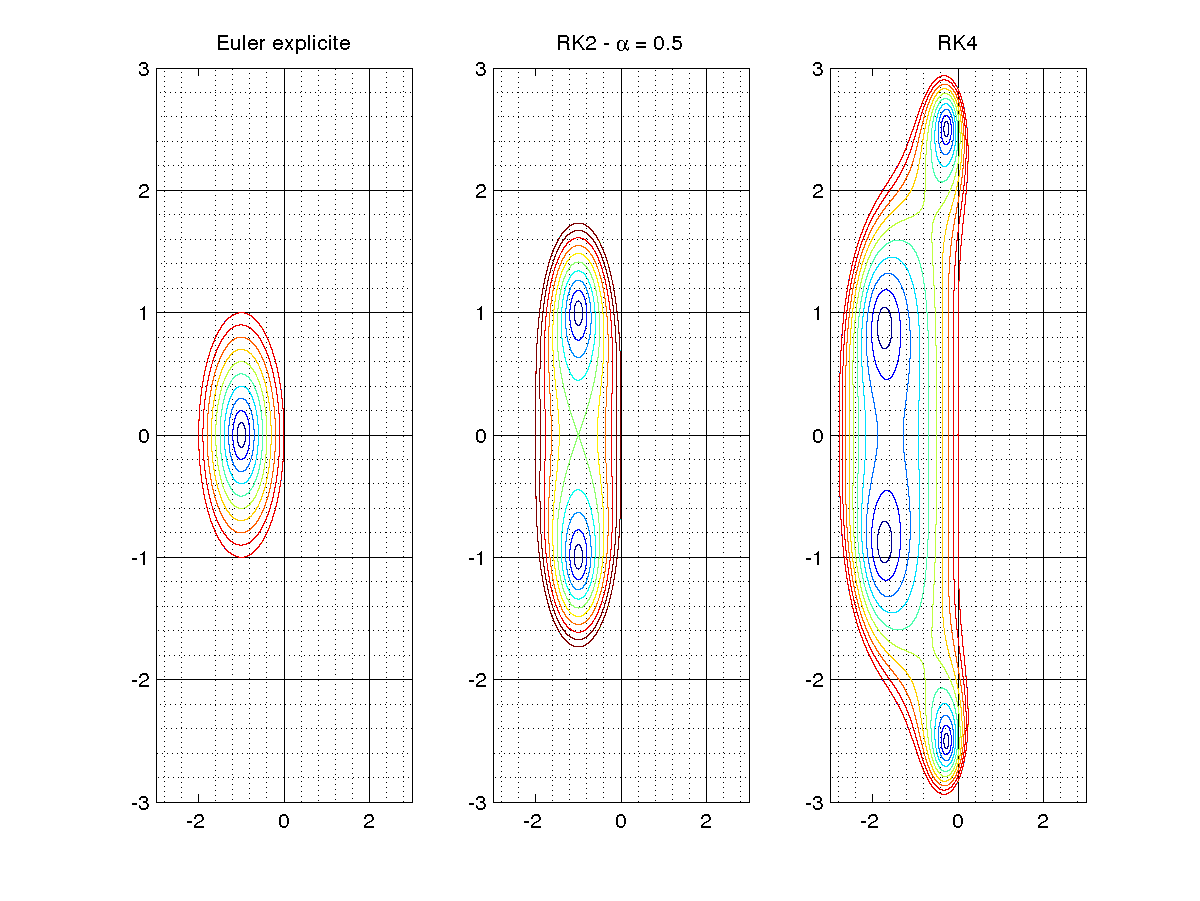
\includegraphics[scale=0.3]{rk_stab.png}
\caption{zone de stabilité de certaines méthodes de Runge-Kutta explicites}
\end{center}
\end{figure}

\end{frame}



% ********************************************************************************
\section{Equation d'advection}
\begin{frame}{Equation d'advection}
\begin{block}{Objectif :}
Obtenir un code de résolution de 
$$\dfrac{\partial h}{\partial t} + \mathbf{c} \cdot \nabla h = 0$$
sur la sphère (+ CI).
\end{block}

Notations : 
\begin{itemize}
\item $(\lambda, \theta)$ : coordonnées longitude-latitude.
\item $(\lambda', \theta')$ : l'axe Nord-Sud est tourné d'un angle $\alpha$.
\end{itemize}
\end{frame}

\begin{frame}{Algorithme}
\begin{block}{}
Résolution basée sur RK4 (explicite à l'ordre 4) et les schémas compacts à l'ordre 4
\end{block}

\begin{enumerate}
\item $K_1 = - \mathbf{c} \cdot \nabla_T h^n$,\\
\item $K_2 = - \mathbf{c} \cdot \nabla_T \left( h^n + \frac{\Delta t}{2} K_1 \right)$,\\
\item $K_3 = - \mathbf{c} \cdot \nabla_T \left( h^n + \frac{\Delta t}{2} K_2 \right)$,\\
\item $K_4 = - \mathbf{c} \cdot \nabla_T \left( h^n + \frac{\Delta
  t}{2} K_4 \right)$,\\
\item \textbf{Assemblage :} $h^{n+1} = h^n + \frac{\Delta t}{6}
  \left(K_1 + 2 K_2 + 2 K_3 + K_4  \right)$
\end{enumerate}

\end{frame}



\subsection{Bump instationnaire}
\begin{frame}{Test de Williamson et al. (1992)}

On impose la vitesse $\mathbf{c} = u \mathbf{e}_{\lambda} + v \mathbf{e}_{\theta}$ par 
\begin{itemize}
\item $u = u_0 \left( cos \theta cos \alpha + sin \theta cos \lambda sin \alpha \right)$
\item $v = - u_0 \left( sin \lambda sin \alpha \right)$
\end{itemize}

\begin{exampleblock}{}
Existence et unicité par la méthode des caractéristiques.
\end{exampleblock}

\begin{block}{}
La condition initiale est transportée sans déformation sur la sphère.
\end{block}
\end{frame}


\begin{frame}
\begin{columns}
\column{0.45\textwidth}
Ce que l'on cherche à avoir...

\begin{figure}
\href{run:ref_7364055200_test_0.avi}{\includegraphics[scale=0.25]{ref_7364055200_solexacte_test_0.png}} 
\caption{Test 0 : Bump en rotation}
\end{figure}

\column{0.45\textwidth}
Ce que l'on observe...

\begin{figure}
\href{run:ref_7363895058_test_0.avi}{\includegraphics[scale=0.25]{ref_7364055200_solexacte_test_0.png}} 
\caption{Test 0 : Bump en rotation - 40 mailles par face - CFL=0.9}
\end{figure}
\end{columns}

\pause
\begin{alertblock}{}
Apparitions d'ondes parasites...
\end{alertblock}
\end{frame}




\subsection{Filtrage numérique}
\begin{frame}{Filtrage Numérique( Redonnet - 2001)}
\begin{alertblock}{Problème}
Présence d'ondes parasites provoquant des erreurs importantes dans la
résolution de l'équations.

$\Rightarrow$ Eliminer les ondes parasites grace à un filtre numérique
\end{alertblock}

$\overline{h}$ : signal filtré issu du signal $h$ :

$$\overline{h}_i = \sum_{p=0}^P f_p \left( h_{i+p} + h_{i-p} \right)$$

Par transformée de Fourier :

$$\hat{\overline{h}} = \underbrace{2 \sum_{p=0}^P f_i cos(\theta)}_{\mathcal{F}(\theta)} \hat{h}$$

\end{frame}

\begin{frame}
Pour éliminer les hautes fréquences et conserver un maximum
d'information, on impose :

$$\partial_{\theta}^{(k)}\mathcal{F} ( \theta ) = \delta_{k,0} \text{ pour } k=0,1,...$$

ainsi que :

$$\mathcal{F} ( \pi ) = 0$$

\textbf{Exemple :} filtre à l'ordre 2

$$\overline{h}_i = \dfrac{1}{2}h_i + \dfrac{1}{4}\left( h_{i+1} +
h_{i-1} \right) $$

\end{frame}

\subsection{\'Etude du cas 1D périodique}
\begin{frame}{Stabilité pour }
Etude sur le cas 1D périodique :
$$
\left \{
\begin{array}{r @{=} l}
\dfrac{\partial h}{\partial t} + c \dfrac{\partial h}{\partial x} & 0\\
h(t,0) & h(t,1)\\
h(0,x) & h_0(x)\\
\end{array}
\right.
$$
Après discrétisation et passage en Fourier:
$$\hat{h}^{n+1} = a(\lambda, \theta) \hat{h}^n$$
avec $\lambda = c \Delta t / \Delta x$ (CFL) et $\theta = \Delta x \xi
$
On définit la CFL maximale par :
$$CFL = max  \{  \lambda \in \mathbb{R} \text{ s. t. } \forall
\theta \in \left[ 0, \pi \right] \text{  } | a( \lambda, \theta ) |
\leq 1 \}$$
Si $\lambda \leq CFL$, le schéma est stable.
\end{frame}

\begin{frame}
Effet du filtre sur la condition CFL :

\begin{columns}
\column{0.45\textwidth}
\begin{center}
\begin{tabular}{cc}
Filtre & CFL\\
\hline
\hline
Pas de filtre & $1.6330$\\
\hline
ordre 10 & $1.6883$\\
\hline
ordre 8 & $1.7114$\\
\hline
ordre 6 & $1.7485$\\
\hline
ordre 4 & $1.8156$\\
\hline
ordre 2 & $1.9749$
\end{tabular}
\end{center}

\column{0.45\textwidth}
\begin{figure}
\begin{center}
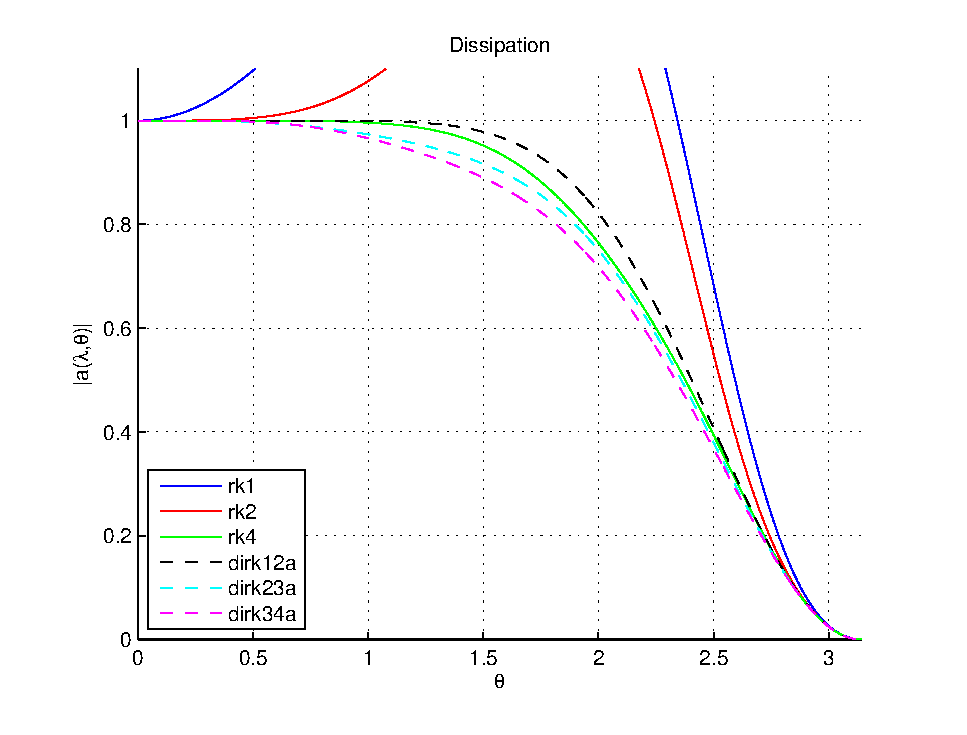
\includegraphics[scale=0.35]{filtre.eps}
\caption{$|a(\lambda, \theta)|$ avec $\lambda = 0.9$}
\end{center}
\end{figure}

\end{columns}

\end{frame}



\subsection{Résultats Numériques}
\begin{frame}{Résultats Numériques}
\begin{columns}
\column{0.45\textwidth}

\begin{figure}
\href{run:ref_7363895782_test_0.avi}{\includegraphics[scale=0.25]{ref_7364056891_normerreur_test_0.png}} 
\caption{Test 0 : Bump en rotation - 40 mailles par face - CFL=0.9 -
  Filtre à l'ordre 2 }
\end{figure}

\column{0.45\textwidth}
\begin{figure}
\href{run:ref_7363896161_test_0.avi}{\includegraphics[scale=0.25]{ref_7364055200_normerreur_test_0.png}} 
\caption{Test 0 : Bump en rotation - 40 mailles par face - CFL=0.9 -
  Filtre à l'ordre 10 }
\end{figure}
\end{columns}
\end{frame}



% ********************************************************************************
\section{Test de Nair et Jablonowski}
\subsection{Présentation}
\begin{frame}{Test de Nair et Jablonowski (2007)}
Deux familles de test :
\begin{itemize}
\item Test de déplacements sans déformations (ex : Williamson et
  al. (1992))\\
\item Test de déformation sans déplacement (ex :  Nair et Machenhauer (2001))
\end{itemize}

\begin{block}{Idée}
Construire un test déformant un vortex et le déplacant le long de la sphère.
\end{block}
\end{frame}

\subsection{Résultats}
\begin{frame}{Résultats Numériques}
\begin{columns}
\column{0.45\textwidth}
test de déformation et de déplacement.
\begin{itemize}

\item $\mathbf{c}$ et $h_0$ donnés,

\item Formation d'une "tempête" (vortex) se déplacant le long d'un cercle sur la sphère.
\end{itemize}


\column{0.45\textwidth}

\begin{figure}
\href{run:ref_7363145849_test_2.avi}{\includegraphics[scale=0.25]{14-Oct-2015_normerreur_test_2.png}} 
\caption{Test 3 : Vortex instationnaire - 40 mailles par face - CFL=0.9}
\end{figure}
\end{columns}
\end{frame}

\begin{frame}

Observation de l'erreur relative :

$$e_2^n = max_{\text{face}} \dfrac{ \| h^n_{i,j} - h(\mathbf{x}_{i,j}, t^n ) \|_2 }{\| h(\mathbf{x}_{i,j}, t^n ) \|_2}$$

\begin{figure}
\begin{tabular}{ccc}
Nombre de points par face & $max_n |e_2^n|$ & estimation de l'ordre \\
\hline
\hline
$41$ & $9.7386 (-2)$ & - \\
\hline 
$51$ & $5.0160 (-2)$ & $3.0399$ \\
\hline
$61$ & $2.6157 (-3)$ & $3.6365$ \\
\hline
$81$ & $8.3722 (-4)$ & $4.0173$ \\
\hline
$101$ & $3.4524 (-4)$ & $4.0143$\\
\hline
$151$ & $6.9199 (-5)$ & $3.9966$
\end{tabular}
\caption{Analyse de convergence du test 3 - $cfl = 0.7$}
\end{figure}

\end{frame}

% ********************************************************************************
\section{Conclusion}
\begin{frame}{Conclusion et perspectives}
\begin{block}{Bilan :}
\begin{itemize}
\item Méthode rapide (Solveurs rapides existants) et précise (ordre 4),\\
\item Bons résultats sur des tests variés,\\
\end{itemize}
\end{block}

\begin{block}{Perspective :}
\begin{itemize}
\item Résolution de LSWE,\\
\item Construction de méthodes implicites,\\
\item Etude sur la conservation de la matière (avec Brice Portenelle).
\end{itemize}
\end{block}


\end{frame}




\section*{}
\begin{frame}
\begin{center}
Merci de votre attention :)
\end{center}
\end{frame}


\end{document}
